\documentclass[aspectratio=169]{beamer}
\usepackage[utf8]{inputenc}
\usepackage[T1]{fontenc}
\usepackage{tikz}
\usepackage{hyperref}
\usepackage{pgfplots}
\usepackage{pgfpages}

\pgfplotsset{compat=1.17}
\setbeameroption{show notes on second screen}
% \pgfpagesuselayout{2 on 1}[a4paper,border shrink=10mm]

\usetheme[darkmode, nofooterlogo]{pureminimalistic}
% \renewcommand{\pageword}{}
\renewcommand{\logotitle}{}
\renewcommand{\logoheader}{}
\renewcommand{\logofooter}{}
\usepackage[backend=biber, doi=false, maxbibnames=2, maxcitenames=2, style=numeric, sorting=none, url=false, eprint=false]{biblatex}
\addbibresource{bibliography.bib}
\usepackage{appendixnumberbeamer}
\renewcommand{\appendixname}{\texorpdfstring{\translate{appendix}}{appendix}}

\title[Debugging of RxJS-based Applications]{Getting rid of the \texttt{console.log}:\\Debugging of RxJS-based Applications}
\author{Manuel Alabor and Markus Stolze}
\institute{OST in Rapperswil, Switzerland}
\date{\today}

\begin{document}

\maketitle

\note[itemize] {
    \item Welcome everyone
    \item I am Manuel
    \item Frontend Software Engineer
    \item Currently TypeScript, React, RxJS
    \item Master Student
    \item Research Topic: Debugging for Reactive Programming -> RxJS
    \item -> Going to tell why this topic
}

\section{Introduction}

\subsection{Why?}

\begin{frame}[fragile]{Reactive Programming for the Web}
    \centering
    \begin{figure}
        \centering
        
\includegraphics[height=\textheight/2]{figures/rxjs-logo.png}
        \caption{RxJS \cite{rxjs}}
        \label{fig:rxjs}
    \end{figure}
\end{frame}

\note[itemize] {
    \item What is RxJS?
    \item One of the larger representatives
    \item RP with JavaScript
    \item You might heard of Angular \cite{angualrrxjs} backed by Google
    \item Angular is based on RxJS
    \item All the things we love about RP: Check
    \item All the things we... dont love about RP: Check
}

\begin{frame}[fragile]{Debugging: First Intuition}
    \begin{figure}[H]
        \centering
        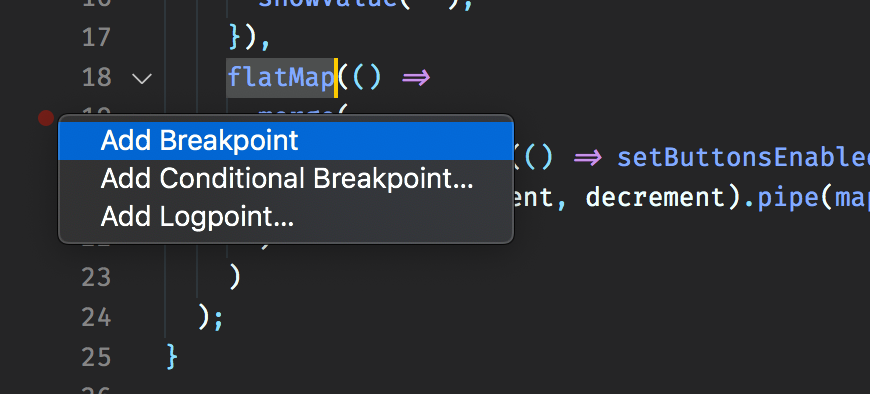
\includegraphics[height=\textheight/2]{figures/add-breakpoint.png}
        \caption{Add a Breakpoint}
    \end{figure}
\end{frame}

\note[itemize] {
    \item How to debug a problem? Well...
    \item Add a breakpoint
    \item Imperative programming debugging
    \item Helps sometimes (lambda functions, ...)
    \item Often useless (stack traces, program step controls...)
    \item What else?
}

\begin{frame}[fragile]{Debugging: The Reality}
    \begin{figure}[H]
        \centering
        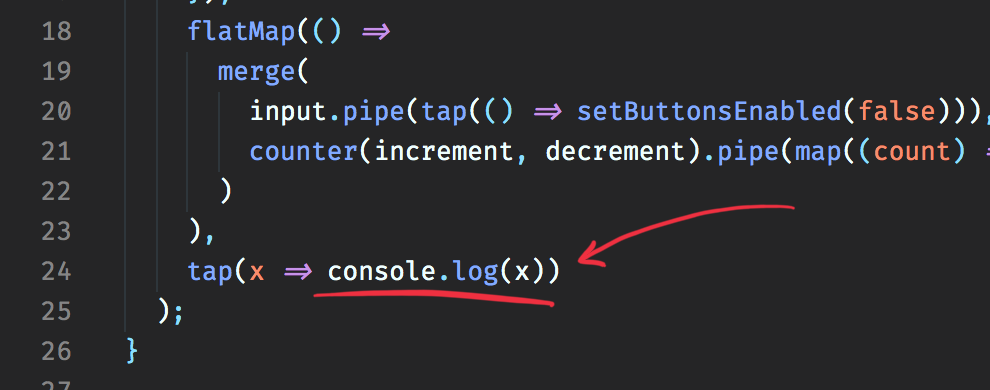
\includegraphics[height=\textheight/2]{figures/consolelog.png}
        \caption{Add Trace Logs}
    \end{figure}
\end{frame}

\note[itemize] {
    \item After some time with RxJS
    \item Stuff gets more complex
    \item Debugging === Trace Logs
    \item Sprinkle log statements throughout the program
    \item Hope to get the right hint
    \item Remove (hopefully) everything again
}

\begin{frame}[fragile]{Debugging: Can this be it?}
    \begin{figure}[H]
        \centering
        
\includegraphics[height=\textheight/2]{figures/person-shrugging_1f937.png}
        \caption{\tiny{Source: \url{https://emojipedia.org/person-shrugging/}}}
    \end{figure}
\end{frame}

\note[itemize] {
    \item Frustration -> Reason Research topic
    \item There are good concepts and solutions for RP debugging
    \item Reactive Debugger, Scala \cite{10.1145/2884781.2884815}
    \item Improved logging tools rxjs-spy \cite{rxjsspy}
    \item Visualizers rxviz \cite{rxviz}
    \item Visualizers rxfiddle \cite{10.1145/3180155.3180156}
    \item But why does nobody seem to use them?
    \item Why unpopular?
    \item -> Research Questions
}


\subsection{Research Questions}
\begin{frame}[fragile]{Research Questions}
    \begin{enumerate}
        \vfill\item[RQ1] \textbf{What challenges} do software engineers face when debugging RxJS-based applications?
        \vfill\item[RQ2] How can the \textbf{experience} of software engineers during the debugging process of RxJS-based applications \textbf{be improved}?
        \vfill\item[\color{gray}{RQ3}] \color{gray}{What is the \textbf{impact of proposed solutions} on the debugging experience of software engineers?}
    \end{enumerate}
\end{frame}

\note[itemize] {
    \item First: Collect and Validate information
    \item Interviews and War Story Reports
    \item Validate this data in an observational study
    \item Second: Propose a solution to improve
    \item Third: Implement and validate solution
    \item Not part of this work
    \item Already started with in current iteration
}


\section{Interviews and War Stories}

\subsection{Interviews}

\begin{frame}[fragile]{One-to-One Interviews}
	\begin{vfilleditems}
		\item Interviewed five \textbf{Engineers}
		\item How do they \textbf{use} Reactive Programming?
		\item What do they \textbf{like},
		\item ... and what \textbf{dislike} about it?
	\end{vfilleditems}
\end{frame}

\note[itemize] {
    \item We were interested in the overall, ...
    \item the good ...
    \item and bad experiences
    \item Not yet debugging specific
    \item Recruited through personal network
    \item Talked to five engineers
    \item 4 RxJS, 1 Scala Akka Streams
    \item Most knew RxJS through Angular
}

\begin{frame}{Quotes}
    \begin{vfilleditems}
		\item[\Large{``}] \textit{[Reactive Programming is] a good way for \textbf{composing} multiple data sources.}
		\item[\Large{``}] \textit{In \textbf{99\%} of all cases, I add \textbf{console.log} statements [\dots] trying to understand what's happening.}
	\end{vfilleditems}
\end{frame}

\note[itemize] {
    \item All interviewees were overall positive to RP
    \item All value RP for complex data \textbf{dependencies}
    \item and \textbf{transformations}
    \item Concrete Quote about console log
    \item Off the record: ``Debugging RP?''
    \item ... well, then you are f***
} 

\subsection{War Stories}
\begin{frame}[fragile]{Call for ``War Stories''}
    \begin{figure}[H]
        \centering
        
\includegraphics[height=0.6\textheight]{figures/tweet-interview.png}
        \caption{\tiny{Source: \url{https://twitter.com/swissmanu/status/1242429409208029185}}}
    \end{figure}
\end{frame}

\note[itemize] {
    \item After first "overall" data collection
    \item Interested in specific data about RxJS Debugging
    \item Twitter and direct-email
    \item 5 replies
    \item RxJS core team member
    \item Google developer experts
    \item Fin Tech Engineers
}

\begin{frame}[fragile]{Report Extracts}
	\begin{vfilleditems}
		\item Traditional debugging utilities are \textbf{seldom sufficient}
		\item Tendency to \textbf{manual} code \textbf{modifications}:
		\begin{vfilleditems}
		    \item Add \textbf{trace logs} with \texttt{console.log}
		    \item \textbf{Extract} code parts to \textbf{sand boxed} environments
		\end{vfilleditems}
	\end{vfilleditems}
\end{frame}

\note[itemize] {
    \item Again: Common practice to modify code
    \item Not only trace logs
    \item Extraction of code parts to extraneous tools
    \item Visualizers rx-viz \cite{rxviz}
    \item Code sandboxes StackBlitz
    \item Try to use debugger
    \item Debuggers often not that useful
}

\subsection{Insights}

\begin{frame}[fragile]{Key Take Aways}
    \begin{columns}[T]
        \begin{column}{.6\linewidth}
            \vspace{3em}
            \begin{itemize}
                \item The ``\textbf{to hammer a screw}''-problem\bigskip
                \item Tendency to \textbf{manual} code \textbf{modifications}\bigskip
                \item Rather \textbf{negative} experience with debugging RxJS-based applications
	        \end{itemize}
        \end{column}
        \begin{column}{.4\linewidth}
            \begin{figure}
                \centering
                
\includegraphics[width=.7\linewidth]{figures/hammer-screw.jpeg}
                \caption{\tiny{Source: Manuel Alabor}}
            \end{figure}
        \end{column}
    \end{columns}
\end{frame}

\note[itemize] {
    \item Traditional debugger feels wrong
    \item Ask a question which they cannot answer (hammer/screw) -> Stack trace
    \item Fallback to manual code modification
    \item Trace log statements
    \item Extract pieces to sandboxes
    \item Overall: Pessimistic view on debugging RxJS RP
    \item Based on this:
    \item Study to validate this...
    \item Hypothesis coming up:
}


\section{Observational Study}
\subsection{Study Design}

\begin{frame}[fragile]{Hypothesis}
    \begin{vfilleditems}
        \item[\Large{``}] If software engineers must solve an RxJS-based problem, then they \textbf{will instrument the code manually} in order to understand its behavior.
    \end{vfilleditems}
\end{frame}

\note[itemize] {
    \item Manual intervention repeating theme
    \item Both Interviews and War Stories
    \item Thats why focus on this in validation study
    \item Dont care what kind (logs vs extraction)
}

\begin{frame}{Study Design}
    \begin{vfilleditems}
        \item \textbf{Observational Study}
        \item \textbf{Briefing} upfront for every subject
        \item \textbf{Uncontrolled} Environment
        \item \textbf{Remote} moderation and execution
        \item ``After Action'' \textbf{Survey}
    \end{vfilleditems}
\end{frame}

\note[itemize] {
    \item Remotely conducted observational study
    \item Execution on subjects computer
    \item Individual dev environment
    \item Mimic "Daily dev routine"
    \item Interested in "How would you tackle RxJS debugging"
    \item Two problems, 25 minutes each
    \item ~1h total
    \item Unattended survey afterwards -> RxJS experience data
}

\begin{frame}{Problem 1: Example}
    \begin{columns}[b]
        \begin{column}{.5\linewidth}
            \begin{figure}
                \centering
                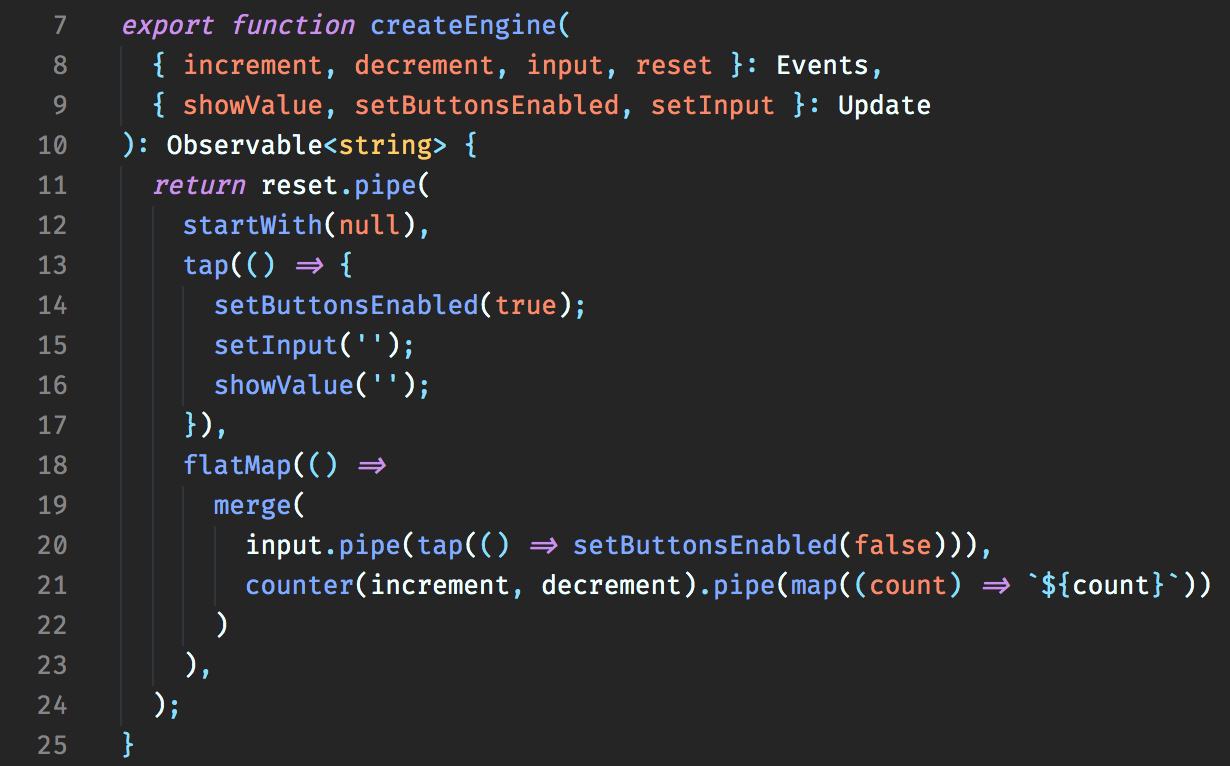
\includegraphics[width=.9\linewidth]{figures/problem1-code.png}
                \caption{RxJS Observable}
            \end{figure}
        \end{column}
        \begin{column}{.5\linewidth}
            \begin{figure}
                \centering
                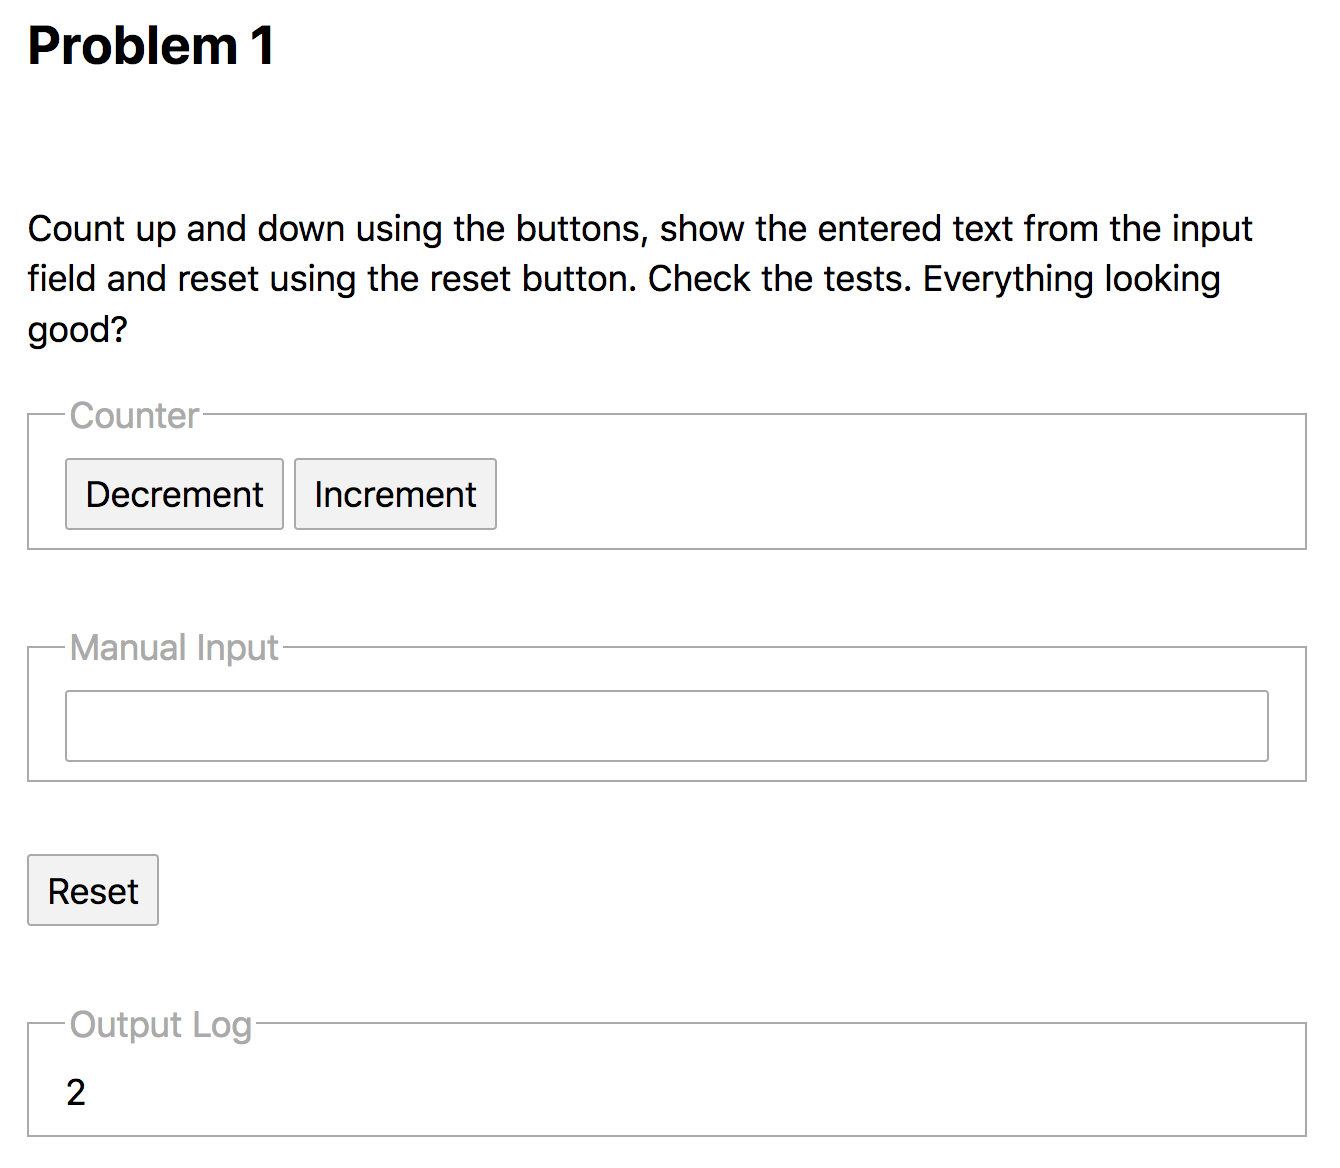
\includegraphics[width=.9\linewidth]{figures/problem1-ui.png}
                \caption{User Interface}
            \end{figure}
        \end{column}
    \end{columns}
\end{frame}

\note[itemize] {
    \item A problem consisted of:
    \item Provided: \textbf{Code}, \textbf{Unit Tests}, \textbf{UI}
    \item Task: Identify and Resolve Bugs
    \item Task: "Speak out loud"
    \item Of course: we did not care IF they actually resolve a problem
    \item Collect as much data how subjects debug
}

\subsection{Study Execution}
\begin{frame}{Subject Population}
    \begin{vfilleditems}
        \item \textbf{Four} professional software engineers
        \item Two currently \textbf{work} with RxJS
        \item Three have \textbf{two or more years} of \textbf{experience} with RxJS
        \item One of them uses RxJS to develop \textbf{backend applications}
    \end{vfilleditems}
\end{frame}

\note[itemize] {
    \item Four engineers recruited from personal network
    \item All use RxJS for frontend development
    \item Only one for backend
    \item Experienced population; most >2y
    \item All: Trace logs
    \item Two: Specialized loggers
    \item Three: Debugger
}

\subsection{Study Results}

\begin{frame}[fragile]{Observed Debugging Techniques}
    \begin{figure}
        \centering
        \begin{tikzpicture}
            \begin{axis}[
                    height=0.6\textheight,
                    width=0.8\linewidth,
                    xbar,
                    xtick={0,1,2,3,4},
                    xlabel={\# of Subjects},
                    symbolic y coords={Add. Tools,Debugger,Trace Logs},
                    ytick=data,
                    enlarge y limits=0.5,
                    enlargelimits=0.15,
                    nodes near coords, nodes near coords align={horizontal}
                ]
                \addplot[
                        fill=pureminimalistic@text@red,
                        draw=pureminimalistic@text@red
                    ]
                    coordinates {
                        (0,Add. Tools) (4,Trace Logs) (2,Debugger) 
                    };
            \end{axis}
        \end{tikzpicture}
    \end{figure}
\end{frame}

\note[itemize] {
    \item All modified/augmented source code manually
    \item -> Trace logs
    \item Two tried traditional debugging
    \item No one extracted code
    \item No one used additional tools
    \item One told afterwards: Would have been their next step
    \item Based on experiment data: Hypothesis is correct
}

\section{Conclusion}

\begin{frame}[fragile]{Interpretation}
    \begin{vfilleditems}
        \item Engineers \textbf{know} RP debugging tools, but \textbf{do not use} them
        \item Engineers use \textbf{imperative}, but actually require ``\textbf{reactive}'' debuggers
        \item \textbf{Manual intervention} is the ``\textbf{last resort}''
    \end{vfilleditems}
\end{frame}

\note[itemize] {
    \item Interviews + War Stories + Study = ?
    \item 7 of 14 peers know specific RxJS debugging tools
    \item But they dont use them
    \item Instead: Traditional tools \textbf{easily accessible}
    \item Final way to go:
    \item Trace logs and code extraction
}

\begin{frame}[fragile]{Answer}
    \begin{enumerate}
        \item[\color{gray}{RQ1}] \color{gray}{What challenges do software engineers face when debugging RxJS-based applications?}
        \vfill\item[\Large{``}] \color{white}{The most significant challenge software engineers face [\dots] is to know \textbf{when} they should apply \textbf{what tool} to resolve their current problem in the \textbf{most efficient} way.}
    \end{enumerate}
\end{frame}

\note[itemize] {
    \item Challenge: What tool, when and how
    \item Often: The "next best" as we saw: Traditional tools
    \item Often: Modify code
    \item Less often: Specific tools
    \item What can we do about it?
    \item Answer question 2
}

\begin{frame}[fragile]{Answer}
    \begin{enumerate}
        \item[\color{gray}{RQ2}] \color{gray}{How can the experience of software engineers during the debugging process of RxJS-based applications be improved?}
        \vfill\item[\Large{``}] \color{white}{[\dots] \textbf{improve} the \textbf{experience} of debugging [\dots] by providing RP specific debugging utilities where software engineers expect them the most: \textbf{Fully integrated} [\dots] their IDE [\dots]}
    \end{enumerate}
\end{frame}

\note[itemize] {
    \item Improve the dev user experience
    \item Lower the boundary to use the right tool
    \item At the right time
    \item Integrate the right tools where they are expected the most
    \item Example: Async Stack Traces in Google Chrome \cite{chromeasync}
}

\section{Future Work}

\begin{frame}[fragile]{Future Work}
    \begin{vfilleditems}
        \item \textbf{Propose} and \textbf{implement} solution to \textbf{prevent} manual code \textbf{modification}
        \item \textbf{Evaluate} proposal on \textbdf{effectiveness} to answer RQ3
    \end{vfilleditems}
\end{frame}

\note[itemize] {
    \item Wraps up our plans for the future
    \item Work on a concrete prototype
    \item Find solution for trace log problem
    \item Without manual intervention
    \item Validate effectiveness and answer RQ3
}

\begin{frame}[fragile]{Sneak Preview}
    \begin{figure}[H]
        \centering
        \includegraphics[height=0.6\textheight]{figures/tweet-rxjs-debugging-extension.png}
        \caption{\tiny{Source: \url{https://twitter.com/swissmanu/status/1313412280072232960}}}
    \end{figure}
\end{frame}

\note[itemize] {
    \item Small sneak preview
    \item Things are progressing
    \item Thank you for your time and attention!
}

\begin{frame}[plain, noframenumbering]
  \centering
  \vfill
  {\fontsize{40}{50}\selectfont\color{white}{Q \& A}}
  \vfill
\end{frame}

\note[itemize] {
    \item Happy for input
    \item Happy to answer questions
}

\appendix
\begin{frame}[allowframebreaks]{References}
	\printbibliography
\end{frame}

\end{document}